
%% bare_jrnl_compsoc.tex
%% V1.4b
%% 2015/08/26
%% by Michael Shell
%% See:
%% http://www.michaelshell.org/
%% for current contact information.
%%
%% This is a skeleton file demonstrating the use of IEEEtran.cls
%% (requires IEEEtran.cls version 1.8b or later) with an IEEE
%% Computer Society journal paper.
%%
%% Support sites:
%% http://www.michaelshell.org/tex/ieeetran/
%% http://www.ctan.org/pkg/ieeetran
%% and
%% http://www.ieee.org/

%%*************************************************************************
%% Legal Notice:
%% This code is offered as-is without any warranty either expressed or
%% implied; without even the implied warranty of MERCHANTABILITY or
%% FITNESS FOR A PARTICULAR PURPOSE! 
%% User assumes all risk.
%% In no event shall the IEEE or any contributor to this code be liable for
%% any damages or losses, including, but not limited to, incidental,
%% consequential, or any other damages, resulting from the use or misuse
%% of any information contained here.
%%
%% All comments are the opinions of their respective authors and are not
%% necessarily endorsed by the IEEE.
%%
%% This work is distributed under the LaTeX Project Public License (LPPL)
%% ( http://www.latex-project.org/ ) version 1.3, and may be freely used,
%% distributed and modified. A copy of the LPPL, version 1.3, is included
%% in the base LaTeX documentation of all distributions of LaTeX released
%% 2003/12/01 or later.
%% Retain all contribution notices and credits.
%% ** Modified files should be clearly indicated as such, including  **
%% ** renaming them and changing author support contact information. **
%%*************************************************************************


% *** Authors should verify (and, if needed, correct) their LaTeX system  ***
% *** with the testflow diagnostic prior to trusting their LaTeX platform ***
% *** with production work. The IEEE's font choices and paper sizes can   ***
% *** trigger bugs that do not appear when using other class files.       ***                          ***
% The testflow support page is at:
% http://www.michaelshell.org/tex/testflow/


\documentclass[10pt,journal,compsoc]{IEEEtran}
%
% If IEEEtran.cls has not been installed into the LaTeX system files,
% manually specify the path to it like:
% \documentclass[10pt,journal,compsoc]{../sty/IEEEtran}

\usepackage{graphicx}
\usepackage{color}
\usepackage{multirow}
\usepackage{listings}
\usepackage{url}
\usepackage{balance}
\usepackage{mathtools}
\DeclarePairedDelimiter{\ceil}{\lceil}{\rceil}

\newif\ifdraft
\drafttrue
%\draftfalse                                                                              
\ifdraft
\newcommand{\zhaonote}[1]{{\textcolor{cyan}    { ***Zhao:      #1 }}}
\newcommand{\note}[1]{ {\textcolor{red}    {\bf #1 }}}
\newcommand{\franknote}[1]{{\textcolor{green}    { ***Frank:      #1 }}}
\newcommand{\evannote}[1]{{\textcolor{blue}    {***Evan:      #1}}}
\else
\newcommand{\zhaonote}[1]{}
\newcommand{\franknote}[1]{}
\newcommand{\evannote}[1]{}
\newcommand{\note}[1]{}
\fi

\lstset{language=java, numbers=left, numberstyle=\tiny\color{black}, numbersep=3pt, escapeinside={\$}, basicstyle=\footnotesize\ttfamily, escapeinside={\%*}{*)}}

% Some very useful LaTeX packages include:
% (uncomment the ones you want to load)


% *** MISC UTILITY PACKAGES ***
%
%\usepackage{ifpdf}
% Heiko Oberdiek's ifpdf.sty is very useful if you need conditional
% compilation based on whether the output is pdf or dvi.
% usage:
% \ifpdf
%   % pdf code
% \else
%   % dvi code
% \fi
% The latest version of ifpdf.sty can be obtained from:
% http://www.ctan.org/pkg/ifpdf
% Also, note that IEEEtran.cls V1.7 and later provides a builtin
% \ifCLASSINFOpdf conditional that works the same way.
% When switching from latex to pdflatex and vice-versa, the compiler may
% have to be run twice to clear warning/error messages.






% *** CITATION PACKAGES ***
%
\ifCLASSOPTIONcompsoc
  % IEEE Computer Society needs nocompress option
  % requires cite.sty v4.0 or later (November 2003)
  \usepackage[nocompress]{cite}
\else
  % normal IEEE
  \usepackage{cite}
\fi
% cite.sty was written by Donald Arseneau
% V1.6 and later of IEEEtran pre-defines the format of the cite.sty package
% \cite{} output to follow that of the IEEE. Loading the cite package will
% result in citation numbers being automatically sorted and properly
% "compressed/ranged". e.g., [1], [9], [2], [7], [5], [6] without using
% cite.sty will become [1], [2], [5]--[7], [9] using cite.sty. cite.sty's
% \cite will automatically add leading space, if needed. Use cite.sty's
% noadjust option (cite.sty V3.8 and later) if you want to turn this off
% such as if a citation ever needs to be enclosed in parenthesis.
% cite.sty is already installed on most LaTeX systems. Be sure and use
% version 5.0 (2009-03-20) and later if using hyperref.sty.
% The latest version can be obtained at:
% http://www.ctan.org/pkg/cite
% The documentation is contained in the cite.sty file itself.
%
% Note that some packages require special options to format as the Computer
% Society requires. In particular, Computer Society  papers do not use
% compressed citation ranges as is done in typical IEEE papers
% (e.g., [1]-[4]). Instead, they list every citation separately in order
% (e.g., [1], [2], [3], [4]). To get the latter we need to load the cite
% package with the nocompress option which is supported by cite.sty v4.0
% and later. Note also the use of a CLASSOPTION conditional provided by
% IEEEtran.cls V1.7 and later.





% *** GRAPHICS RELATED PACKAGES ***
%
\ifCLASSINFOpdf
  % \usepackage[pdftex]{graphicx}
  % declare the path(s) where your graphic files are
  % \graphicspath{{../pdf/}{../jpeg/}}
  % and their extensions so you won't have to specify these with
  % every instance of \includegraphics
  % \DeclareGraphicsExtensions{.pdf,.jpeg,.png}
\else
  % or other class option (dvipsone, dvipdf, if not using dvips). graphicx
  % will default to the driver specified in the system graphics.cfg if no
  % driver is specified.
  % \usepackage[dvips]{graphicx}
  % declare the path(s) where your graphic files are
  % \graphicspath{{../eps/}}
  % and their extensions so you won't have to specify these with
  % every instance of \includegraphics
  % \DeclareGraphicsExtensions{.eps}
\fi
% graphicx was written by David Carlisle and Sebastian Rahtz. It is
% required if you want graphics, photos, etc. graphicx.sty is already
% installed on most LaTeX systems. The latest version and documentation
% can be obtained at: 
% http://www.ctan.org/pkg/graphicx
% Another good source of documentation is "Using Imported Graphics in
% LaTeX2e" by Keith Reckdahl which can be found at:
% http://www.ctan.org/pkg/epslatex
%
% latex, and pdflatex in dvi mode, support graphics in encapsulated
% postscript (.eps) format. pdflatex in pdf mode supports graphics
% in .pdf, .jpeg, .png and .mps (metapost) formats. Users should ensure
% that all non-photo figures use a vector format (.eps, .pdf, .mps) and
% not a bitmapped formats (.jpeg, .png). The IEEE frowns on bitmapped formats
% which can result in "jaggedy"/blurry rendering of lines and letters as
% well as large increases in file sizes.
%
% You can find documentation about the pdfTeX application at:
% http://www.tug.org/applications/pdftex






% *** MATH PACKAGES ***
%
%\usepackage{amsmath}
% A popular package from the American Mathematical Society that provides
% many useful and powerful commands for dealing with mathematics.
%
% Note that the amsmath package sets \interdisplaylinepenalty to 10000
% thus preventing page breaks from occurring within multiline equations. Use:
%\interdisplaylinepenalty=2500
% after loading amsmath to restore such page breaks as IEEEtran.cls normally
% does. amsmath.sty is already installed on most LaTeX systems. The latest
% version and documentation can be obtained at:
% http://www.ctan.org/pkg/amsmath





% *** SPECIALIZED LIST PACKAGES ***
%
%\usepackage{algorithmic}
% algorithmic.sty was written by Peter Williams and Rogerio Brito.
% This package provides an algorithmic environment fo describing algorithms.
% You can use the algorithmic environment in-text or within a figure
% environment to provide for a floating algorithm. Do NOT use the algorithm
% floating environment provided by algorithm.sty (by the same authors) or
% algorithm2e.sty (by Christophe Fiorio) as the IEEE does not use dedicated
% algorithm float types and packages that provide these will not provide
% correct IEEE style captions. The latest version and documentation of
% algorithmic.sty can be obtained at:
% http://www.ctan.org/pkg/algorithms
% Also of interest may be the (relatively newer and more customizable)
% algorithmicx.sty package by Szasz Janos:
% http://www.ctan.org/pkg/algorithmicx




% *** ALIGNMENT PACKAGES ***
%
%\usepackage{array}
% Frank Mittelbach's and David Carlisle's array.sty patches and improves
% the standard LaTeX2e array and tabular environments to provide better
% appearance and additional user controls. As the default LaTeX2e table
% generation code is lacking to the point of almost being broken with
% respect to the quality of the end results, all users are strongly
% advised to use an enhanced (at the very least that provided by array.sty)
% set of table tools. array.sty is already installed on most systems. The
% latest version and documentation can be obtained at:
% http://www.ctan.org/pkg/array


% IEEEtran contains the IEEEeqnarray family of commands that can be used to
% generate multiline equations as well as matrices, tables, etc., of high
% quality.




% *** SUBFIGURE PACKAGES ***
%\ifCLASSOPTIONcompsoc
%  \usepackage[caption=false,font=footnotesize,labelfont=sf,textfont=sf]{subfig}
%\else
%  \usepackage[caption=false,font=footnotesize]{subfig}
%\fi
% subfig.sty, written by Steven Douglas Cochran, is the modern replacement
% for subfigure.sty, the latter of which is no longer maintained and is
% incompatible with some LaTeX packages including fixltx2e. However,
% subfig.sty requires and automatically loads Axel Sommerfeldt's caption.sty
% which will override IEEEtran.cls' handling of captions and this will result
% in non-IEEE style figure/table captions. To prevent this problem, be sure
% and invoke subfig.sty's "caption=false" package option (available since
% subfig.sty version 1.3, 2005/06/28) as this is will preserve IEEEtran.cls
% handling of captions.
% Note that the Computer Society format requires a sans serif font rather
% than the serif font used in traditional IEEE formatting and thus the need
% to invoke different subfig.sty package options depending on whether
% compsoc mode has been enabled.
%
% The latest version and documentation of subfig.sty can be obtained at:
% http://www.ctan.org/pkg/subfig




% *** FLOAT PACKAGES ***
%
%\usepackage{fixltx2e}
% fixltx2e, the successor to the earlier fix2col.sty, was written by
% Frank Mittelbach and David Carlisle. This package corrects a few problems
% in the LaTeX2e kernel, the most notable of which is that in current
% LaTeX2e releases, the ordering of single and double column floats is not
% guaranteed to be preserved. Thus, an unpatched LaTeX2e can allow a
% single column figure to be placed prior to an earlier double column
% figure.
% Be aware that LaTeX2e kernels dated 2015 and later have fixltx2e.sty's
% corrections already built into the system in which case a warning will
% be issued if an attempt is made to load fixltx2e.sty as it is no longer
% needed.
% The latest version and documentation can be found at:
% http://www.ctan.org/pkg/fixltx2e


%\usepackage{stfloats}
% stfloats.sty was written by Sigitas Tolusis. This package gives LaTeX2e
% the ability to do double column floats at the bottom of the page as well
% as the top. (e.g., "\begin{figure*}[!b]" is not normally possible in
% LaTeX2e). It also provides a command:
%\fnbelowfloat
% to enable the placement of footnotes below bottom floats (the standard
% LaTeX2e kernel puts them above bottom floats). This is an invasive package
% which rewrites many portions of the LaTeX2e float routines. It may not work
% with other packages that modify the LaTeX2e float routines. The latest
% version and documentation can be obtained at:
% http://www.ctan.org/pkg/stfloats
% Do not use the stfloats baselinefloat ability as the IEEE does not allow
% \baselineskip to stretch. Authors submitting work to the IEEE should note
% that the IEEE rarely uses double column equations and that authors should try
% to avoid such use. Do not be tempted to use the cuted.sty or midfloat.sty
% packages (also by Sigitas Tolusis) as the IEEE does not format its papers in
% such ways.
% Do not attempt to use stfloats with fixltx2e as they are incompatible.
% Instead, use Morten Hogholm'a dblfloatfix which combines the features
% of both fixltx2e and stfloats:
%
% \usepackage{dblfloatfix}
% The latest version can be found at:
% http://www.ctan.org/pkg/dblfloatfix




%\ifCLASSOPTIONcaptionsoff
%  \usepackage[nomarkers]{endfloat}
% \let\MYoriglatexcaption\caption
% \renewcommand{\caption}[2][\relax]{\MYoriglatexcaption[#2]{#2}}
%\fi
% endfloat.sty was written by James Darrell McCauley, Jeff Goldberg and 
% Axel Sommerfeldt. This package may be useful when used in conjunction with 
% IEEEtran.cls'  captionsoff option. Some IEEE journals/societies require that
% submissions have lists of figures/tables at the end of the paper and that
% figures/tables without any captions are placed on a page by themselves at
% the end of the document. If needed, the draftcls IEEEtran class option or
% \CLASSINPUTbaselinestretch interface can be used to increase the line
% spacing as well. Be sure and use the nomarkers option of endfloat to
% prevent endfloat from "marking" where the figures would have been placed
% in the text. The two hack lines of code above are a slight modification of
% that suggested by in the endfloat docs (section 8.4.1) to ensure that
% the full captions always appear in the list of figures/tables - even if
% the user used the short optional argument of \caption[]{}.
% IEEE papers do not typically make use of \caption[]'s optional argument,
% so this should not be an issue. A similar trick can be used to disable
% captions of packages such as subfig.sty that lack options to turn off
% the subcaptions:
% For subfig.sty:
% \let\MYorigsubfloat\subfloat
% \renewcommand{\subfloat}[2][\relax]{\MYorigsubfloat[]{#2}}
% However, the above trick will not work if both optional arguments of
% the \subfloat command are used. Furthermore, there needs to be a
% description of each subfigure *somewhere* and endfloat does not add
% subfigure captions to its list of figures. Thus, the best approach is to
% avoid the use of subfigure captions (many IEEE journals avoid them anyway)
% and instead reference/explain all the subfigures within the main caption.
% The latest version of endfloat.sty and its documentation can obtained at:
% http://www.ctan.org/pkg/endfloat
%
% The IEEEtran \ifCLASSOPTIONcaptionsoff conditional can also be used
% later in the document, say, to conditionally put the References on a 
% page by themselves.




% *** PDF, URL AND HYPERLINK PACKAGES ***
%
%\usepackage{url}
% url.sty was written by Donald Arseneau. It provides better support for
% handling and breaking URLs. url.sty is already installed on most LaTeX
% systems. The latest version and documentation can be obtained at:
% http://www.ctan.org/pkg/url
% Basically, \url{my_url_here}.





% *** Do not adjust lengths that control margins, column widths, etc. ***
% *** Do not use packages that alter fonts (such as pslatex).         ***
% There should be no need to do such things with IEEEtran.cls V1.6 and later.
% (Unless specifically asked to do so by the journal or conference you plan
% to submit to, of course. )


% correct bad hyphenation here
\hyphenation{op-tical net-works semi-conduc-tor}


\begin{document}
%
% paper title
% Titles are generally capitalized except for words such as a, an, and, as,
% at, but, by, for, in, nor, of, on, or, the, to and up, which are usually
% not capitalized unless they are the first or last word of the title.
% Linebreaks \\ can be used within to get better formatting as desired.
% Do not put math or special symbols in the title.
\title{Scientific Computing Meets Big Data Technology: An Astronomy Use Case}
%
%
% author names and IEEE memberships
% note positions of commas and nonbreaking spaces ( ~ ) LaTeX will not break
% a structure at a ~ so this keeps an author's name from being broken across
% two lines.
% use \thanks{} to gain access to the first footnote area
% a separate \thanks must be used for each paragraph as LaTeX2e's \thanks
% was not built to handle multiple paragraphs
%
%
%\IEEEcompsocitemizethanks is a special \thanks that produces the bulleted
% lists the Computer Society journals use for "first footnote" author
% affiliations. Use \IEEEcompsocthanksitem which works much like \item
% for each affiliation group. When not in compsoc mode,
% \IEEEcompsocitemizethanks becomes like \thanks and
% \IEEEcompsocthanksitem becomes a line break with idention. This
% facilitates dual compilation, although admittedly the differences in the
% desired content of \author between the different types of papers makes a
% one-size-fits-all approach a daunting prospect. For instance, compsoc 
% journal papers have the author affiliations above the "Manuscript
% received ..."  text while in non-compsoc journals this is reversed. Sigh.

\author{\begin{tabular}{cccc}
{Zhao~Zhang} & {Kyle~Barbary} & {Frank~Austin~Nothaft} & {Evan~R.~Sparks} \\
{Oliver~Zahn} & {Michael~J.~ Franklin} & {David~A.~Patterson} & {Saul~Perlmutter}
\end{tabular}% <-this % stops a space
%\\%\and % use '\and' if you need 'another row' of author names
%\begin{tabular}{c}
%$^*$ AMPLab, University of California, Berkeley \\
%$^\circ$ Berkeley Institute for Data Science, University of California, Berkeley\\
%$^\dagger$ Berkeley Center for Cosmological Physics, University of California, Berkeley\\
%$^\ddagger$ ASPIRE Lab, University of California, Berkeley \\
%\end{tabular}
\IEEEcompsocitemizethanks{
\IEEEcompsocthanksitem Zhao~Zhang and Michael~J.~Franklin are with
the AMPLab and Berkeley Institute for Data Science, UC Berkeley.\protect
% note need leading \protect in front of \\ to get a newline within \thanks as
% \\ is fragile and will error, could use \hfil\break instead.
\IEEEcompsocthanksitem Frank~Austin~Nothaft and David~A.~Patterson are with the AMP and ASPIRE Labs, UC Berkeley.
\IEEEcompsocthanksitem Evan~R.~Sparks is with the AMPLab, UC Berkeley.
\IEEEcompsocthanksitem Kyle~Barbary, Oliver~Zahn, and Saul~Perlmutter are with the
Berkeley Institute for Data Science and Berkeley Center for Cosmological Physics, UC Berkeley.
}% <-this % stops an unwanted space
%\thanks{Manuscript received April 19, 2005; revised August 26, 2015.}
}

% note the % following the last \IEEEmembership and also \thanks - 
% these prevent an unwanted space from occurring between the last author name
% and the end of the author line. i.e., if you had this:
% 
% \author{....lastname \thanks{...} \thanks{...} }
%                     ^------------^------------^----Do not want these spaces!
%
% a space would be appended to the last name and could cause every name on that
% line to be shifted left slightly. This is one of those "LaTeX things". For
% instance, "\textbf{A} \textbf{B}" will typeset as "A B" not "AB". To get
% "AB" then you have to do: "\textbf{A}\textbf{B}"
% \thanks is no different in this regard, so shield the last } of each \thanks
% that ends a line with a % and do not let a space in before the next \thanks.
% Spaces after \IEEEmembership other than the last one are OK (and needed) as
% you are supposed to have spaces between the names. For what it is worth,
% this is a minor point as most people would not even notice if the said evil
% space somehow managed to creep in.



% The paper headers
%\markboth{Journal of \LaTeX\ Class Files,~Vol.~14, No.~8, August~2015}%
%{Shell \MakeLowercase{\textit{et al.}}: Bare Demo of IEEEtran.cls for Computer Society Journals}
% The only time the second header will appear is for the odd numbered pages
% after the title page when using the twoside option.
% 
% *** Note that you probably will NOT want to include the author's ***
% *** name in the headers of peer review papers.                   ***
% You can use \ifCLASSOPTIONpeerreview for conditional compilation here if
% you desire.



% The publisher's ID mark at the bottom of the page is less important with
% Computer Society journal papers as those publications place the marks
% outside of the main text columns and, therefore, unlike regular IEEE
% journals, the available text space is not reduced by their presence.
% If you want to put a publisher's ID mark on the page you can do it like
% this:
%\IEEEpubid{0000--0000/00\$00.00~\copyright~2015 IEEE}
% or like this to get the Computer Society new two part style.
%\IEEEpubid{\makebox[\columnwidth]{\hfill 0000--0000/00/\$00.00~\copyright~2015 IEEE}%
%\hspace{\columnsep}\makebox[\columnwidth]{Published by the IEEE Computer Society\hfill}}
% Remember, if you use this you must call \IEEEpubidadjcol in the second
% column for its text to clear the IEEEpubid mark (Computer Society jorunal
% papers don't need this extra clearance.)



% use for special paper notices
%\IEEEspecialpapernotice{(Invited Paper)}



% for Computer Society papers, we must declare the abstract and index terms
% PRIOR to the title within the \IEEEtitleabstractindextext IEEEtran
% command as these need to go into the title area created by \maketitle.
% As a general rule, do not put math, special symbols or citations
% in the abstract or keywords.
\IEEEtitleabstractindextext{%
\begin{abstract}
\zhaonote{revised with Kira-v2 SE performance}
Scientific analyses commonly compose multiple single-process programs into a dataflow.
An end-to-end dataflow of single-process programs is known as a many-task application.
Typically, HPC tools are used to parallelize these analyses.
In this work, we investigate an alternate approach that uses Apache Spark---a modern platform for data intensive computing---to parallelize many-task applications.
Using Apache Spark, we implement Kira, a flexible and distributed astronomy image processing toolkit. 
We then use the Kira toolkit to implement the Kira SE application for extracting sources from astronomy images.
Using Kira SE as a case study, we study the programming flexibility, dataflow richness, scheduling capacity and performance
of Apache Spark running on the EC2 cloud.
By exploiting data locality, Kira SE achieves a 4.1$\times$ speedup over an equivalent C program when analyzing a 1TB
dataset using 512 cores on the Amazon EC2 cloud.
Furthermore, we show that by leveraging software originally designed for big data infrastructure, we are able to use the Amazon EC2 cloud to achieve a 1.8$\times$ speedup over  
the C implementation running on the NERSC Edison supercomputer, when holding core count constant.
Using the same implementation of Kira SE, a 128-core EC2 cloud deployment that uses Spark Streaming can achieve second-scale latency with a 
sustained throughput of $\sim$600~MB/s.
Our experience with Kira demonstrates that data intensive computing platforms like Apache Spark are a performant alternative for many-task scientific applications.  

\end{abstract}

% Note that keywords are not normally used for peerreview papers.
\begin{IEEEkeywords}
Distributed Computing, Data Processing, Astronomy, Many-Task Applications
\end{IEEEkeywords}}


% make the title area
\maketitle


% To allow for easy dual compilation without having to reenter the
% abstract/keywords data, the \IEEEtitleabstractindextext text will
% not be used in maketitle, but will appear (i.e., to be "transported")
% here as \IEEEdisplaynontitleabstractindextext when the compsoc 
% or transmag modes are not selected <OR> if conference mode is selected 
% - because all conference papers position the abstract like regular
% papers do.
\IEEEdisplaynontitleabstractindextext
% \IEEEdisplaynontitleabstractindextext has no effect when using
% compsoc or transmag under a non-conference mode.



% For peer review papers, you can put extra information on the cover
% page as needed:
% \ifCLASSOPTIONpeerreview
% \begin{center} \bfseries EDICS Category: 3-BBND \end{center}
% \fi
%
% For peerreview papers, this IEEEtran command inserts a page break and
% creates the second title. It will be ignored for other modes.
\IEEEpeerreviewmaketitle



\IEEEraisesectionheading{\section{Introduction}\label{sec:introduction}}
% Computer Society journal (but not conference!) papers do something unusual
% with the very first section heading (almost always called "Introduction").
% They place it ABOVE the main text! IEEEtran.cls does not automatically do
% this for you, but you can achieve this effect with the provided
% \IEEEraisesectionheading{} command. Note the need to keep any \label that
% is to refer to the section immediately after \section in the above as
% \IEEEraisesectionheading puts \section within a raised box.





% The very first letter is a 2 line initial drop letter followed
% by the rest of the first word in caps (small caps for compsoc).
% 
% form to use if the first word consists of a single letter:
% \IEEEPARstart{A}{demo} file is ....
% 
% form to use if you need the single drop letter followed by
% normal text (unknown if ever used by the IEEE):
% \IEEEPARstart{A}{}demo file is ....
% 
% Some journals put the first two words in caps:
% \IEEEPARstart{T}{his demo} file is ....
% 
% Here we have the typical use of a "T" for an initial drop letter
% and "HIS" in caps to complete the first word.
\IEEEPARstart{D}{ramatic} increases in dataset sizes have made data processing a major bottleneck for scientific research in many disciplines, such as astronomy, genomics, social science, and neuroscience.
Researchers frequently start with a C or Fortran program that is optimized for processing a small amount of data on a single-node workstation and then use distributed processing frameworks to improve processing capacity. Examples include the Montage astronomy image mosaic application~\cite{jacob09}, the sequence alignment tool BLAST~\cite{altschul90}, and high energy physics histogram analysis~\cite{ekanayake08}.
These applications are known as many-task applications because they comprise many small single-process tasks that are connected by dataflow patterns~\cite{raicu08}.

Scientists have used dedicated workflow systems (e.g., HTCondor~\cite{litzkow88}), parallel frameworks (e.g., the Message Passing Interface, MPI~\cite{gropp96}), and more recently the data processing system Hadoop~\cite{HADOOP} to build these applications. Each approach has its own advantages such as provenance tracking, high scalability, and automated parallelism. However, these approaches also have shortcomings such as limited programming flexibility, lack of fault-tolerance, or a rigid programming model.


Apache Spark~\cite{zaharia12} was designed to support fast iterative data analyses on very large datasets by relying on an in-memory data model that allows
for the caching of intermediate results. By using a directed acyclic graph~(DAG) to describe parallel tasks, 
Spark provides resilience against transient failures by replaying computational lineage
and can optimize for data locality when scheduling tasks.
These features have made Apache Spark a widely used distributed computing platform for machine learning~\cite{gonzalez14, sparks13} and computational science~\cite{freeman14, massie13, nothaft15}, and
make Spark a natural platform for executing many-task applications.

In this work, we investigate how to leverage Apache Spark for many-task applications.
We study this question in the context of Kira, an astronomy image processing toolkit~\cite{zhang15}.
We use the Kira SE application to evaluate the programming flexibility, dataflow richness,
and scheduling capacity of Spark. Kira SE performs source extraction, a common astronomy application that identifies point sources in an image. We evaluate Kira SE's performance by comparing against
an equivalent C implementation that is parallelized using HPC tools. Leveraging an multi-language analytics platform like Apache Spark provides several advantages for many-task applications:
\begin{enumerate}
\item Spark can use existing astronomy libraries written in Python and C.
This allows astronomers to reuse existing libraries to build new analysis functionality.
\item Spark supports a broad range of dataflow patterns such as pipeline, broadcast, scatter, gather, reduce, allgather,
and alltoall (shuffle). This broad dataflow pattern support can be used to optimize the data transfer between computation stages.
\item Spark's broad support for underlying file systems allows Kira to process data stored in a distributed file system such as HDFS~\cite{shvachko10}, 
as well as data stored in HPC-style shared file systems such as GlusterFS~\cite{davies13} or Lustre~\cite{donovan03}, or cloud blob stores like Amazon S3 and Microsoft DataLake.
\item The Kira toolkit also inherits Spark's fault tolerance mechanism, which is a feature missing from MPI~\cite{gropp96}.
\item \zhaonote{This is new} The same Kira implementation can leverage other components of the Berkeley Data Analytic Stack (BDAS), e.g., Spark Streaming~\cite{zaharia13}.
\end{enumerate}

Our experiments show that Spark is capable of managing $O(10^6)$ tasks and that Kira SE runs 4.1$\times$ faster than an equivalent C program when using a shared file system on the Amazon EC2 cloud with the 1TB Data Release 7 from the Sloan Digital Sky Survey~\cite{york00}. We also show that running Kira SE in the Amazon EC2 cloud can achieve performance that is 1.8$\times$ faster than that of the equivalent C program running on the NERSC Edison supercomputer.

Our experience with Kira indicates that Big Data platforms such as Apache Spark are a competitive alternative for many-task scientific applications.
We believe this is important, because leveraging such platforms would enable scientists to benefit from the rapid pace of innovation and large range of systems and technologies that are being driven by wide-spread interest in Big Data analytics.
Kira is open source software released under an MIT license and is available from \linebreak \url{https://github.com/BIDS/Kira}.

\section{Background}
\label{sec:Background}

This section reviews the science behind sky surveys, introduces the source extraction kernel, explores engineering requirements, and discusses the origin and usage of Spark.

\subsection{Sky Surveys}

Modern astronomical research is increasingly based around large-scale sky surveys.
Rather than selecting specific targets to study, such a survey will uniformly observe large
swaths of the sky. Example surveys include the Sloan Digital Sky Survey (SDSS)~\cite{york00},
the Dark Energy Survey (DES)~\cite{dark05}, and the Large Synoptic Survey Telescope~(LSST,
\cite{ivezic08}). Enabled by new telescopes and cameras with wide fields of view, these
surveys deliver huge datasets that can be used for many different scientific studies
simultaneously.

In addition to studying the astrophysical properties of many different individual galaxies,
the large scale of these surveys allows scientists to use the distribution of galaxies to
study the biggest contemporary mysteries in astrophysics: dark matter, dark energy, and 
the properties of gravity. These surveys normally include a time component: each patch of the sky is imaged many times,
with observations spread over hours, days, weeks or months. With this repeated imaging,
transient events can be detected via ``difference imaging''. Transients such as supernovae
can be detected in large numbers to better measure dark energy, and the large survey area
often results in the discovery of new, extremely rare, transient phenomena.

\subsection{Source Extraction}
\label{sec:Background-SE}
Source extraction is a key step in astronomical image processing pipelines.
SExtractor~\cite{bertin96} is a widely used C application for source extraction. The source
extraction kernel identifies and extracts point sources of light against the dark background of
a standard telescope image.
%Users need to specify $\sim$40 parameters to run the application. 
Although SExtractor is currently implemented as a monolithic C program for extracting astronomical
objects from images, the application's logic can be divided into 
background estimation, background removal, object detection, and astrometric 
and photometric estimation.

Astronomers can improve extraction accuracy by running multiple iterations of source
extraction. Detected objects are removed after each iteration. While
the original C program contains the required functionality for building this iterative source extractor,
it does not expose the interfaces through the command line. To resolve this issue,
SEP~\cite{barbary2015} reorganizes the code base of SExtractor to expose the core estimation, removal, and detection
functions as a library. SEP provides both C and Python interfaces. Users can then
build the iterative source extractor using SEP primitives. Kira SE is implemented by calling into
the SEP library.

\subsection{Engineering Requirements}
\label{sec:Background-EngReq}

In some experiments---such as experiments that search for supernovae explosions---it is important to process
the images as rapidly as possible. A rapid processing pipeline enables astronomers to trigger follow-up
observations with more sensitive instrumentation before the peak of the supernovae occurs.
High throughput is also needed in large scale
sky survey pipelines that perform real time data analysis, such as the LSST~\cite{ivezic08}.
The LSST uses a 2.4m-wide optical telescope that captures 3.2 billion pixels per
image. This telescope produces approximately 12.8~GB in 39~seconds
for a sustained rate of $\sim$330~MB per second, and a typical night produces 13~TB of data. 
Over the planned 10-year project, the survey is expected produce 60~PB of raw data, which will be consolidated into a 15~PB catalog.
The latency requirements of this pipeline couple with the massive amount of data captured to create a challenging throughput requirement for the 
processing pipeline. 

\subsection{Spark}
Apache Spark is a dataflow-based execution system that provides a functional, collection
oriented API~\cite{zaharia12}. Spark's development was motivated by a need for a
system that could rapidly execute iterative workloads on very large datasets, as is common
in large scale machine learning~\cite{zaharia10}. Spark has
become widely adopted in industry, and academic research groups have used Spark
for the analysis of scientific datasets in areas such as neuroscience~\cite{freeman14} and genomics~\cite{nothaft15}.

Spark is centered around the Resilient Distributed Dataset~(RDD) abstraction~\cite{zaharia12}.
To a programmer, RDDs appear as an immutable collection of independent items that are 
distributed across the cluster. RDDs are immutable and are transformed using a
functional API. Operations on RDDs are evaluated lazily, enabling the system to schedule 
execution and data movement with better knowledge of the operations to be performed than 
systems that immediately execute each stage. Spark provides Scala, Java, and Python programming interfaces.
By default, Spark uses HDFS~\cite{shvachko10} for persistent storage, but
it can process data stored in Amazon S3 or on a shared file system such as
GlusterFS~\cite{davies13} or Lustre~\cite{donovan03}. Spark provides fault tolerance via
lineage-based recomputation. If a partition of data is lost, Spark can recover the data
by re-executing the section of the DAG that computed the lost partition.

\zhaonote{This is new}
Spark implemented streaming data processing using a discretized stream (D-Streams) architecture, which built upon the
RDD abstraction~\cite{zaharia13}.
D-Streams partition data streams into multiple small time intervals, which are transformed using a series of stateless and deterministic operations.
Spark streaming can recover from faults and stragglers at second-scale by using the lineage-based fault tolerance techniques
built into Spark's RDD abstraction. D-Streams are able to achieve second-scale latency when processing streaming data.

\section{Applying Spark to \\ Many-Task Applications}
\label{sec:Capability}

Scientific analysis pipelines are frequently assembled by building a dataflow out of many
single-process programs. Many-task applications arise in scientific research
domains including astronomy, biochemistry, bioinformatics, psychology, economics, climate science,
and neuroscience. In these applications, tasks are typically grouped into stages that are connected by
producer-consumer data sharing relationships. 
A previous survey study~\cite{katz11} identified
seven common dataflow patterns among a group of many-task applications. The patterns
include pipeline, broadcast, scatter, gather,
reduce, allgather, and alltoall. Most many-task applications
can be viewed as stages of independent tasks that are linked by these dataflow patterns.

The map-reduce~\cite{dean04} model uses a similar pattern to schedule jobs. Traditional map-reduce
systems such as Google's MapReduce~\cite{dean04} and Apache Hadoop MapReduce~\cite{HADOOP} 
abstract producer-consumer relationships into a map stage and a reduce stage. These two stages are then
linked by a data shuffle. Although these systems have proved very powerful for processing very
large datasets, the map-reduce API has been criticized as inflexible~\cite{dewitt08}.
Additionally, since jobs are restricted to a single map and reduce phase, tools such as
FlumeJava~\cite{chambers10} are necessary for assembling pipelines of map-reduce jobs. Since
data is spilled to disk at the end of each map and reduce phase, traditional map-reduce platforms perform poorly
on iterative and pipelined workflows~\cite{zaharia12}.

To resolve these problems, second-generation map-reduce execution systems such as
DryadLINQ~\cite{yu08} and Spark~\cite{zaharia12} allow for applications to be decomposed into
DAGs. In these DAGs, nodes represent computation, and the nodes are
linked by dataflows. In Spark, this abstraction is provided by RDDs~\cite{zaharia12}. Table~\ref{tb:Patterns} demonstrates how seven common dataflow patterns can be mapped
to Apache Spark.

\begin{table}[h]
  \begin{center}
  \caption{Dataflow Pattern Primitives in Spark}
    \begin{small}
    \begin{tabular}{ | p{1.8cm} | p{5.5cm} |}
    \hline
    Pattern & Spark primitive \\
    \hline \hline
    Pipeline & RDD.map()  \\ 
    Broadcast & sparkContext.broadcast() \\   
    Scatter & sparkContext.parallelize() \\ 
    Gather & RDD.collect() \\ 
    Reduce & RDD.reduce() \\ 
    Allgather & RDD.collect().broadcast() \\ 
    Alltoall & RDD.reduceByKey() or \\
 & RDD.repartition() \\ 
    \hline
    \end{tabular}
    \end{small}   
  \label{tb:Patterns}     	
  \end{center}
\end{table}

Spark improves upon
Hadoop MapReduce by adding an in-memory processing model that natively supports iterative computation. 
As compared to other DAG based methods such as DryadLINQ, this enables
the efficient execution of chained pipeline stages. In a chained pipeline,
Disk I/O and inter-process communication are only performed before the first stage of the chain, and after the
last stage of the chain. Spark uses communication barriers to synchronize the execution of each stage~\cite{zaharia12}.

\section{Kira Design and Implementation}
\label{sec:Design}

When designing the Kira astronomy image processing toolkit, 
we focused on improving computational performance and I/O cost while providing a flexible programming interface that enables code reuse.

\subsection{Architecture Overview}
\label{sec:Design-Overview}

Kira's overall architecture is shown in Figure~\ref{fig:architecture}. 
Each outer box with rounded corners is a process. A process can be
a Spark Driver, a Spark Worker, or a HDFS daemon (NameNode or DataNode).
Kira runs on top of Spark, which supports a single driver and multiple workers.
The SEP library (shaded inner box) is deployed to all workers nodes. 
The input files are stored in the underlying file system.

\begin{figure}[t]
	\begin{center}
		\includegraphics[width=85mm]{pictures/Kira-Architecture}
		\caption{Overview of Kira's Architecture and Inter-Component Interactions}
		\label{fig:architecture}
  	\end{center}
\end{figure}

To run Kira, we submit the compiled program, the parameters, and library dependencies to the Spark Driver.
The Spark Driver manages control flow, dataflow, and task scheduling 
by coordinating the Spark workers. 
The Spark Driver accesses distributed/parallel file systems for metadata and the I/O operations are distributed across the Spark worker nodes in parallel. 

\zhaonote{talking about two interface}
When running a task, workers perform computation by calling out to the SEP library.
For Spark's native Scala/Java interface, Kira calls the C library through the Java Native Interface~(JNI).
With Spark's Python bindings~(PySpark), Kira calls the C library through the
pre-compiled Python interface provided by the SEP library. 

\subsection{Computation}
\label{sec:Design-Computation}
We considered three approaches when implementing the Source Extractor algorithm in Kira:

\begin{enumerate}
\item We can \textbf{reimplement} the Source Extractor algorithm from scratch.
\item We can connect existing programs as \textbf{monolithic} pieces without changing them.
\item We can reorganize the C-based SExtractor implementation to expose a programmable
\textbf{library} that we call.
\end{enumerate}

While \textbf{reimplementing} the functionality of the C SExtractor code using Spark's Scala API 
would allow us to execute SExtractor in parallel, it would lower the efficiency of the computation 
and would require a significant reimplementation effort.
The \textbf{monolithic} approach would not involve a modification to the original executable. While we could 
integrate with the original codebase at this level, this would lock us in to the hardcoded program logic 
of the original program. 
For example, astronomers can improve extraction accuracy by running multiple iterations of source
extraction with detected sources being removed from the input image after each iteration. 
The original SExtractor contains the required functionality for this iterative process, however, the hardcoded
logic only allows users to run the source extraction once.  
In order to not be locked in to the rigid control flow limitations of the \emph{monolithic} model, 
we instead opt for a \textbf{library}-based model.
This approach allows us to reuse the legacy code base without sacrificing control-flow flexibility.  


\subsection{I/O}
\label{sec:Design-I/O}
The Flexible Image Transport System (FITS)~\cite{wells81} format is a widely adopted file format for astronomy
images. Each FITS file contains ASCII metadata and binary image data.
The FITS format is commonly used by sky surveys, thus Kira must be able to process and export FITS files.
In Kira, one of our goals is to leverage the locality information provided by HDFS. When a file is loaded into 
HDFS, the file is split into blocks that are replicated across machines. When a system such as Spark loads the file, 
HDFS then provides information about which machines have each block of the file. This allows the
scheduler to optimize task placement for data locality.

Kira uses the \texttt{SparkContext.binaryFiles()} API.
This API loads all files within a directory as a sequence of tuples. 
Each tuple contains the file object and a byte stream containing the contents of the file. 
With Spark's Scala interface, we then use the jFITS~\cite{jfits} library to convert these byte streams 
into the FITS objects that users can transform and compute upon. 
In PySpark, we use the Astropy~\cite{astropy13} Python library.

\subsection{Spark Streaming}
\label{sec:Design-Streaming}
Spark streaming can monitor an HDFS directory for new files and process the new files periodically. 
The Python interface of the Spark Streaming 1.6.0 release supports both text files and fixed-length binary records.
We introduce a new streaming interface called \texttt{SparkContext.binaryFileStream()} to read the FITS
files as binary streams. 
Then, the source extraction procedure can be applied to the data by calling batch processing routines.

\section{Programming Kira}
\label{sec:Programming}
The Kira API is described in Table~\ref{tb:Primitives}. 
Background methods are used to estimate and remove the image background. The Extractor
API is used for extracting objects and estimating astrometric and photometric parameters. The Ellipse API offers helper
functions for converting between ellipse representations, and for generating masks that are based on an object's elliptical
shape. The \texttt{sum\_circle()}, \texttt{sum\_ellipse()}, and \texttt{kron\_radius()} methods in the extractor category and all
methods in the ellipse category perform batch processing, where the input coordinates are passed as a three dimensional array. 
With Spark's Scala API, we are able to amortize the cost of each Java Native Interface (JNI) call by processing objects in batches.

\begin{table*}[t]
\begin{center}
\caption{Kira Primitives and Explanation}
\label{tb:Primitives}
\begin{tabular}{ |l|l|l| }
\hline
Group & API & Explanation \\ \hline \hline
\multirow{3}{*}{Background} & makeback() & Builds background from an input image \\
 & backarray() & Returns the background as a 2D array \\
 & subbackarray() & Subtracts a given background from image \\ \hline
\multirow{4}{*}{Extractor} & extract() & Returns objects extracted from the input image \\
 & sum\_circle() & Sums data in circular apertures \\
 & sum\_ellipse() & Sums data in elliptical apertures \\ 
 & kron\_radius() & Calculate iron radius within an ellipse \\ \hline
\multirow{3}{*}{Ellipse} & ellipse\_coeffs() & Converts from ellipse axes and angle to coefficient representations \\
 & ellipse\_axes() & Converts from coefficient representations to ellipse axes and angles \\ 
 & mask\_ellipse() & Masks out certain pixels that fall in a given ellipse \\ \hline
\end{tabular}
\end{center}
\end{table*}

This API allows us to build a source extractor in Kira that is equivalent to the SEP
extractor~\cite{barbary2015}.
Listing~\ref{lst:SE} contains pseudocode describing how to implement a source extractor
using Kira's API. This code uses Spark's \texttt{binaryFiles()} method to load input
files from persistent storage. We then map over each file to convert the FITS data into
a matrix with associated metadata. In the final map stage, we estimates and remove the
background from the matrix. Once the background is removed, we then extract the objects
from the matrix.

\begin{lstlisting}[caption=Objects Extraction Logic, label=lst:SE, linewidth=0.5\textwidth, xleftmargin=2.5ex]
val input_rdd = sparkContext.binaryFiles(src)
val mtx_rdd = input_rdd.map(f => load(f))
val objects_rdd = mtx_rdd.map(m => {
  /* mask is a 2-d array with 
   * the same dimensions as m
   */
  val mask = null
  val bkg = new Background(m, mask)
  val matrix = bkg.subfrom(m)
  val ex = new Extractor
  val objects = ex.extract(matrix))
})
\end{lstlisting}

In Listing~\ref{lst:SE-Iter}, we demonstrate how the Kira API can be used to perform
iterative image refinement. Although the original SExtractor~\cite{bertin96} contains all necessary functionality, 
it is not feasible for users to implement this feature due to the hardcoded program logic . However, since Kira provides
library level bindings, it is easy to implement a multi-stage refinement pipeline.

\begin{lstlisting}[caption=Iterative Objects Extraction Logic, label=lst:SE-Iter, linewidth=0.5\textwidth, xleftmargin=2.5ex]
val input_rdd = sparkContext.binaryFiles(src)
val mtx_rdd = input_rdd.map(f=>load(f))
val objects_rdd = mtx_rdd.(m => {
  /*mask is a 2-d array with 
   *the same size of m
   */
  var mask = null
  var ex = new Extractor   
  for(i <- 0 until 5) {
    var bkg = new Background(m, mask)
    var matrix = bkg.subfrom(m) 
    var objects = ex.extract(matrix)
    mask = mask_ellipse(objects)  
  }
  objects
})
\end{lstlisting}

Listing~\ref{lst:SE-Iter} wraps the source extraction phase from Listing~\ref{lst:SE} in a loop. 
This allows us to update the mask used for extraction, which is used to further refine the extraction
in subsequent iterations.

\section{Tuning Spark}
This section discusses how we configure Spark in terms of parallelism and scheduling to make
Kira SE more efficiently use EC2 computing resources. 

\subsection{Parallelism}

Spark allows for both thread and process parallelism. By default, Spark makes use of
thread-level parallelism by launching a single Java Virtual Machine~(JVM) per worker machine.
Users then specify the number of threads to launch per worker (typically, one thread per core).
However, with Spark's Scala API in Kira SE, neither the jFITS nor the JNI are thread safe. 
To work around this, we configured Spark to support process level parallelism by launching 
a worker instance for each core. 
This configuration may reduce scalability, as it increases the number of workers the driver manages
and can reduce the performance of broadcast operations, as broadcast objects are replicated across workers.
However, our experiments with 512 workers in~\S\ref{sec:Performance} show that Kira's scalability is 
not severely impacted by worker management or broadcast overhead.
The Kira/PySpark implementation is thread safe, and we launch a single Spark worker per machine when running
under PySpark. Each Spark worker then manages the multiple cores on the machine.

\subsection{Scheduling}

Spark's task-scheduling policy aims to maximize data locality by using
delay scheduling~\cite{zaharia10ds}. In this scheduling paradigm, if node $n$ has the data needed
to run job $j$, job $j$ will execute on node $n$ if job $j$ would wait less than a threshold time
$t$ to start. The policy is tunable through three parameters:

\begin{itemize}
\item{spark.locality.wait.process}
\item{spark.locality.wait.node}
\item{spark.locality.wait.rack}
\end{itemize}

These parameters allow users to specify how much time a task will wait before being sent to another
process, node, or rack. For Kira SE, we have found that data balancing can 
impact task distribution, leading to node starvation and a reduction in overall performance.
Loading a 65~GB (11,150 files) dataset from SDSS Data Release 2 to a 16-node HDFS deployment ideally should result in 699 files on each node.
In reality, the number of files on each node varies between 617 and 715.
Enforcing locality with longer {\em spark.locality.wait} time (3000 ms) leads to task distribution imbalance, which makes
Kira SE 4.5\% slower than running with {\em spark.locality.wait} set to 0~ms.
In practice, we set all {\em spark.locality.wait} parameters to zero, so that tasks do not wait for locality.
This setting effectively avoids starvation and improves the overall time-to-solution.

The root cause of the ineffectiveness of delay scheduling is the size of the input files for the Kira SE tasks. 
Each input file is $\sim$6~MB, compared to a typical block size of 64/128~MB~\cite{shvachko10}.
Delay scheduling's parameters let users specify how long a task should wait for locality before getting executed elsewhere.
This waiting time can be viewed as the expected job completion time difference between executing the task with data locality and without locality.
In the Kira SE case, the need for scheduling a task to a node without locality only occurs when there is a possible
starvation if we continue to enforce the locality. Since our input files are small, the cost of doing a remote fetch is low and thus we should only
wait for a short period time~\cite{ananthanarayanan11}. By sweeping the waiting time, we found that not waiting delivered the best performance.
While this result seems to contradict our result in~\S\ref{sec:Performance} that states that Apache Spark outperforms
the HPC solution due to data locality, it is not contradictory because even with no delay scheduling, 
98\% of the tasks scheduled have local data.  Thus the delay scheduling penalty is not needed in this case.   
We have traded a 2\% decrease in locality for a 4.5\% improvement in overall performance.

\section{An HPC Solution}
\label{sec:HPC}
A typical way to parallelize a many-task application like source extractor is to use a scripting language
or MPI to launch multiple tasks concurrently. Figure~\ref{fig:hpc-architecture} shows the architecture
of such a solution.

\begin{figure}[t]
	\begin{center}
		\includegraphics[width=85mm]{pictures/HPC-Architecture}
		\caption{Overview of a Parallel Version of Source Extractor using HPC Tools}
		\label{fig:hpc-architecture}
  	\end{center}
\end{figure}

All the input files are stored in the shared file system, e.g., GlusterFS or Luster. We use a master script
first to read all the input file names, then partition the file names into partitions. After that, the master
script informs the worker scripts on each node to process an independent partition of files in parallel 
in a batch manner.

For GlusterFS, metadata is distributed across the cluster and the metadata query from the master script
communicates with all nodes. The file I/O is done by the worker nodes. Note that unlike HDFS, 
POSIX I/O libraries cannot take advantage of data placement locality during file read/write. While Lustre 
file I/O is similar to GlusterFS, file system metadata is consolidated onto a small set of metadata servers.

\section{Performance}
\label{sec:Performance}
Over the previously implemented Kira with Spark's Scala interface, we migrate to the pySpark Python interface 
for increased uptake in the astronomy community. In the course of this migration, we optimized data layout and took efforts to make zero-copy calls to external libraries, which led to significant performance improvements. To differentiate the two implementations,
we refer to them as Kira-SE-v1 and Kira-SE-v2, respectively.

We compare both of the Kira implementations against the HPC solution that runs
the C code in the SEP library (referred to as the C version in the following text). 
Because all implementations use the same SEP library, Kira SE (both versions) 
perform an identical amount of computation and I/O as the C version.

To understand Spark's overhead, we first compare Kira SE's performance against the C version on a single
machine. Then we fix the problem size and scale Kira SE and the C implementation across a
varying number of machines on EC2 to understand the relative scalability of each approach.
The 1TB experiments demonstrate the difference in performance between Kira SE and the C version
for large dataset processing. Finally, we show some interesting results when running the C
version on the Edison supercomputer that is deployed at the National Energy Research Scientific Computing Center (NERSC).

In all experiments using Amazon's EC2 service, we use m2.4xlarge instances for spinning disks and r3.2xlarge instance for solid state disks.
The m2.4xlarge instance type has eight cores (each running at 2.4GHz), 68~GB RAM, two hard disk drives (HDD), and Gigabit Ethernet. 
We chose this HDD based configuration to give a fair comparison against the Edison supercomputer, which is backed by HDDs. 
An performance study with newer solid state drive (SSD) backed instances is also conducted.
We study the relation of streaming interval and data freshness based on 16 m2.4xlarge instances.
Software configurations are described in the following experiments.
If not stated otherwise, we run each experiment three times, and present the average.
Error bars in the figures are standard deviation of the measurements.

\subsection{Single Machine Performance}
\label{sec:Performance-scaleup}

The purpose of the scale-up experiments is to understand Spark's overhead by running
Kira SE on a single node. 
With Kira-SE-v1, the performance slowdown is caused mainly by Java Virtual Machine (JVM) and JNI overhead.
With Kira-SE-v2, the slowdown is caused by the interaction between the runtime of Scala, Python and C. 
We also wanted to identify the factors that bound Kira SE's performance. 
For both Kira SE and the C implementation, we store data locally in an ext4 file system.

For this experiment, we use a 12GB dataset from the SDSS DR2 survey. The dataset contains
2310 image files and each image is $\sim$6MB.
Figure~\ref{fig:scaleup} shows the relative
performance of Kira SE and the C version for various core counts on a single machine.

\begin{figure}[h]
	\begin{center}
		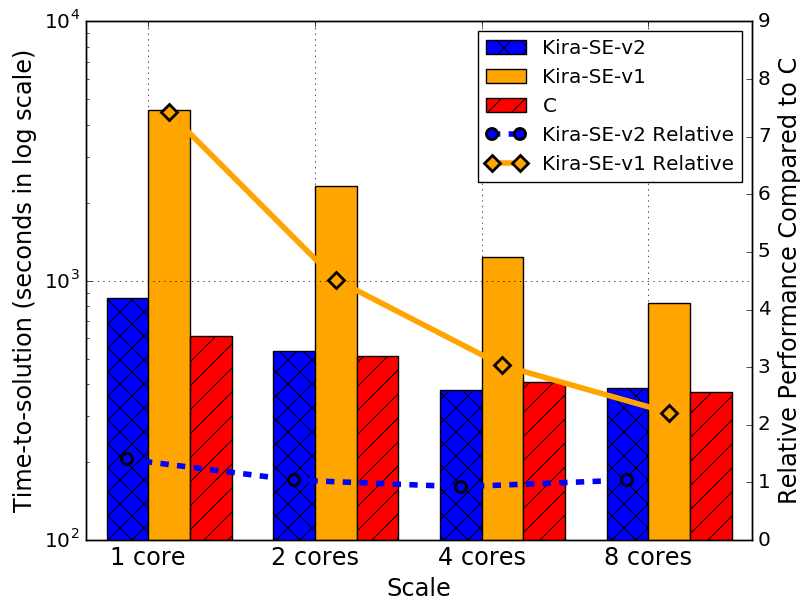
\includegraphics[width=85mm]{pictures/scaleup}
		\caption{Single-Node Scale-Up Performance Comparison between Kira SE and the C Version (Lower is Better) 
		%\evannote{The 4th caption in the legend needs to change from ``pyKira'' to ``Kira-SE-v2 Relative''}
		\label{fig:scaleup}}
  	\end{center}
\end{figure}

\zhaonote{revised with Kira SE v2 performance}
The C version is bound by local disk performance and runtime improves by 65\% when scaling from a single core
to eight cores.
Although Kira-SE-v1 is $7.4\times$ slower than the C implementation
on a single core, Kira-SE-v1 is within $2.2\times$ the performance of the C version when using all eight cores on the node.
Kira-SE-v2 is 39.7\% slower than the C implementation with a single core, while this performance gap
shrinks as the core count increases. And the performance of Kira-SE-v2 converges to the C performance beyond four cores.
The scaling curves indicate that the performance of the approaches begins to converge
as core count increases. At convergence, both of the approaches saturate the local
disk bandwidth.

With a performance breakdown profile, we confirm that the performance improvement of Kira-SE-v2 over
Kira-SE-v1 is attributable to using the SEP-native data layout in our pySpark application as well as the minimized data copy between SEP library and the core C library. That is, by allowing SEP to operate in-place on the images without an expensive pre-process and copy step, we are able to improve Kira's performance dramatically.

We also profile the C implementation with both warm and cold file system caches. When running with a
cold cache, the job completed in 371 seconds while the job completed in 83 seconds when
running with a warm cache. This indicates that 78\% of job execution time is consumed by
I/O (reading and writing data between local disk and memory). Since the C implementation of
SExtractor is disk bound, we believe that it is representative of a data intensive application. 

\subsection{Scale-Out Performance}
\label{sec:Performance-scaleout}

Next, we wanted to understand the strong scaling performance of both Kira SE and the C
implementation. Although Kira-SE-v1 has 2.2$\times$ worse performance when running on
a single machine, we expect that Kira-SE-v1 will achieve better performance at scale due
to disk locality. We expect that this will allow Kira-SE-v1 to outperform the C implementation
on large clusters. 
\zhaonote{revised with Kira-SE-v2 performance}
For Kira-SE-v2, it can be viewed as an improvement combination of locality and native C
computation performance. We expect Kira-SE-v2 to be faster than the C implementation
at all scales.

We use a 65GB dataset from the SDSS DR7 survey that comprises 11,150 image files.
Kira SE was configured to use HDFS as a storage system, while the C version used GlusterFS. 
Both HDFS and GlusterFS are configured with a replication factor of two.

\zhaonote{revised with Kira-SE-v2 performance}
Figure~\ref{fig:scaleout} compares the performance of Kira-SE-v1, Kira-SE-v2, and the C version across
multiple compute nodes in log scale. 
Kira-SE-v1 is 2.7$times$ slower as the C version on eight cores. 
However, the gap between the two implementations decreases as we scale up. 
On 256 cores and 512 cores, Kira-SE-v1 is respectively 5.6\% and 22.4\% faster than the C version.
The Kira-SE-v2 shows a more significant improvement over the C implementation with a speedup of
2.2$\times\sim$3.1$\times$ across scales.
Both the Kira-SE-v1 and Kira-SE-v2 show exhibit near linear scalability.


\begin{figure}[h]
	\begin{center}
		\includegraphics[width=85mm]{pictures/scaleout}
		\caption{Scale-Out Performance Comparison between Kira SE and the C Version in Logarithmic Scale (Lower is Better)
		\label{fig:scaleout}}
  	\end{center}
\end{figure}

\zhaonote{revised with Kira-SE-v2 performance}
The fundamental driver of Kira-SE-v1's and Kira-SE-v2's linear scalability is its consistent local disk
hit ratio, which is the ratio between the number of tasks that access the input file 
on local disk and total number of tasks. Tacking Kira-SE-v2 as an example, Spark and HDFS optimize for data locality during scheduling and achieve a
hit ratio around 98\% with a small standard deviation (around 0.2\%), as shown in Figure~\ref{fig:locality}. 
In contrast, the C implementation's estimated locality hit ratio decreases in half as the cluster size doubles.

\begin{figure}[h]
	\begin{center}
		\includegraphics[width=85mm]{pictures/locality}
		\caption{Locality Hit Ratio (Higher is Better)
		\label{fig:locality}}
  	\end{center}
\end{figure}

In general, a shared file system can be configured in many ways to achieve better
availability, performance, and resilience. To understand the impact of the shared
file system configuration, we compare the performance of Kira SE (time-to-solution)
against four configurations of GlusterFS. The four configurations are
\emph{distributed}, \emph{replicated}, \emph{striped}, and \emph{striped replicated}. 
Table~\ref{tb:gluster-conf} explains the data layout of each configuration.
When possible, we set the replication and striping factors to two.
GlusterFS manages metadata in a distributed manner by spreading metadata across
all available nodes with a hash function. This allows the clients to deterministically
know the location of the metadata of a given file name in the cluster.

\begin{table}[h]
  \begin{center}
  \caption{GlusterFS Configuration Modes and Data Layout}
    \begin{small}
    \begin{tabular}{ | p{1.65cm} | p{6cm} |}
    \hline
    Configuration & Data Layout \\ \hline \hline
    distributed & files are distributed to all nodes without replication  \\ \hline
    replicated & files are distributed to all nodes with a number of replicas specified by the user \\ \hline  
    striped & files are partitioned into a pre-defined number of stripes then distributed to all nodes without replication \\ \hline
    striped replicated & files are partitioned into a pre-defined number of stripes and the stripes are distributed to all nodes with a number of replicas specified by the user \\ \hline
    \end{tabular}
    \end{small}   
  \label{tb:gluster-conf}     	
  \end{center}
\end{table}

We evaluate these configurations using the same dataset as the scale-out experiment. We
select 128 cores and 256 cores as the target scale since it is the transition point in
Figure~\ref{fig:scaleout} where Kira-SE-v1 begins to run faster than the C version. 
As stated previously in~\S\ref{sec:HPC}, the C version performs a two-step process. 
The first step collects and partitions all file paths. We refer to this step as metadata overhead. 
The processing step occurs next, and is where each node processes its own partition.
Figure~\ref{fig:allgluster} compares the performance of Kira-SE-v1, Kira-SE-v2,  and the C version with
profiled metadata overhead.  

\begin{figure}[h]
	\begin{center}
		\includegraphics[width=85mm]{pictures/allgluster}
		\caption{Kira SE Performance Compared to All GlusterFS Configurations (Lower is Better)
		\label{fig:allgluster}}
  	\end{center}
\end{figure}

The C version running in the \emph{distributed} mode outperforms Kira-SE-v1 at both scales. 
However, the \emph{distributed} mode is not practical in a cloud environment since
it has no replication or any other resilience mechanism. Replicating or striping
files introduces extra metadata overhead when we compare the \emph{replicated} mode
to the \emph{distributed} mode. The metadata overhead for each configuration increases
with large scales due to the cost of managing distributed metadata.

Another observation is that striping will further slow down metadata processing, whereas the
processing part takes less time than the \emph{distributed} mode for both scales due
to the doubled probability of accessing half file (with the striping factor of two) in local disk.
Since the input files are $\sim$6MB each, and are always processed by a single task, the
\emph{replicated} mode should be preferred to the \emph{striped replicated} mode.

\zhaonote{revised with Kira-SE-v2 performance}
When running on 256 cores, Kira-SE-v1 outperforms all GlusterFS configurations except for the (impractical) \emph{distributed}
mode. When comparing to the \emph{distributed} mode, Kira-SE-v1 delivers comparable performance, as it is 18\% slower. 
In our experiments with the 1TB dataset in Section~\ref{sec:1TB-EC2}, 
Kira-SE-v1 outperforms the \emph{distributed} mode.

\zhaonote{revised with Kira-SE-v2 performance}
As expected, Kira-SE-v2 improves the performance significantly with speedups of 2.1$\times$ and 1.8 $\times$
compared to the \emph{distributed} mode on 128 cores and 256 cores, respectively.

\subsection{1TB Dataset Performance}
\label{sec:Performance-1TB}

We select a 1TB dataset from the SDSS DR7 survey, which is comprised of 176,938 image files. 
With this experiment, we seek to answer the following questions: 

\begin{itemize}
\item Can Kira scale to process a 1TB dataset?
\item What is the relative performance of Kira compared to the HPC version on the Amazon EC2 cloud?
\item How does Kira SE performance compare to the HPC version on a supercomputer?
\end{itemize}

\subsubsection{Cloud}
\label{sec:1TB-EC2}
\zhaonote{revised with Kira-SE-v2 performance}
We configure GlusterFS in \emph{replicated} and \emph{distributed} modes and compare 
Kira-SE-v1's and Kira-SE-v2's performance against the C implementation. 
Kira-SE-v1 runs $1.1\times$ and $1.3\times$ faster than the C version running on top of
GlusterFS configured in \emph{distributed} mode on 256 cores and 512 cores respectively. 
Using the more practical \emph{replicated} configuration of GlusterFS, Kira-SE-v1 is $2.3\times$ and $2.5\times$ faster. 
On the other hand, Kira-SE-v2 runs $2.5\times$ and $2.0\times$ faster than the impractical \emph{distributed} mode on 256 cores and 512 cores, respectively.
Kira-SE-v2 is also $4.1\times\sim5.2\times$ faster than the \emph{replicated} mode.
A detailed breakdown of the performance is shown in Figure~\ref{fig:1tb-ec2}.
The C version in \emph{distributed} mode is slower due to the node starvation that is introduced by our HPC solution.
The C version in \emph{replicated} mode slows down $2.2\times$ than that in \emph{distributed} mode because the directory metadata query
is dramatically slower ($13.4\times$), and the additional replica for each output file and associated metadata update introduces a slowdown
of $1.4\times$.

\begin{figure}[t]
	\begin{center}
		\includegraphics[width=85mm]{pictures/1TB-EC2}
		\caption{Kira SE Performance with 1TB Input Compared to the C Version Running on GlusterFS on EC2 (Lower is Better)
		\label{fig:1tb-ec2}}
  	\end{center}
\end{figure}

\zhaonote{revised with Kira-SE-v2 performance}
Compared to the experiment with the 65GB dataset in Section~\ref{sec:Performance-scaleout},
Kira-SE-v2 processes $15.9\times$ more data in $16.3\times$ more time. If we discount the Spark
startup time, we can see that Kira-SE-v2 scales linearly in relation to the data size.

\zhaonote{revised with Kira-SE-v2 performance}
The overall throughput of Kira-SE-v2 is 1,335~MB/second, which is $4.0\times$ greater than necessary
to support the upcoming Large Synoptic Survey Telescope (LSST), as discussed in
Section~\ref{sec:Background-EngReq}. This high throughput enables real-time image processing.

\subsubsection{Supercomputer}

Many astronomers have access to supercomputers and believe that
supercomputers outperform commodity clusters for data-intensive applications.
To examine this belief, we compare Kira-SE-v1 and Kira-SE-v2 on the Amazon cloud versus the performance of
the C version running on the NERSC Edison supercomputer, a Cray XC 30 System. We use
the Lustre file system which provides a peak throughput of 48GB/s. Each compute
node of Edison is equipped with a 24-core Ivy Bridge processor, with a 2.4GHz clock rate.
This is comparable to the CPU speed of the Amazon EC2 m2.4xlarge instance (eight vCPUs of
Intel Xeon E5-2665, each running at 2.4GHz). The experiments on Edison run on 21
nodes (a total of 504 cores) in the Cluster Compatibility Mode~(CCM)
while Kira SE uses 64 nodes (512 cores) on EC2. The Cray CCM provides a 
standard Linux cluster environment with services such as ssh, rsh, nscd, and ldap which 
are not supported in Cray's native mode.
Figure~\ref{fig:1tb-edison} shows the measurements.

\begin{figure}[h]
	\begin{center}
		\includegraphics[width=85mm]{pictures/1TB-edison}
		\caption{Kira SE Performance with 1TB Input Compared to the C Version Running on NERSC Edison Supercomputer (Lower is Better)
		\label{fig:1tb-edison}}
  	\end{center}
\end{figure}

Kira-SE-v1 delivers a comparable performance to that of the C version on Edison. 
While the Kira-SE-v2 achieves a $1.8\times$ speedup compared to that of Edison performance.
During the experiments, we see that the C version performance varies significantly with an 
average time-to-solution of 1,388.9~seconds and a standard deviation of 520.5~seconds. 
These results clearly fall into two classes. The first class has an average time-to-solution of 937.8~seconds
with a standard deviation of 69.5~seconds. The second class has an average time-to-solution 
of 1840.1~seconds with a standard deviation of 248.7~seconds. A further analysis shows that we are only 
using 0.4\% of the computing resources of the Edison machine. In the first class, the sustained
I/O bandwidth is 1.0 GB/s, which is 2.1\% of the I/O bandwidth available on the file system.
While in the second class, the sustained I/O bandwidth is down to 0.5GB/s.
Since the Edison cluster scheduler only schedules a single job per compute node, computing resources 
are completely isolated. Thus, we can reason that, it is the I/O network resource or the file system 
that causes the performance variance. 

\zhaonote{revised with Kira-SE-v2 performance}
On the other hand, Kira-SE-v2 is able to accelerate the performance by 1.8x with an average time-to-solution of
767.4~seconds and a standard deviation of 10.9~seconds. The stable performance of both version of Kira SE
can be attributed to exploiting data locality: both the Kira implementations move the I/O from network
to local disk access, which gives a higher I/O bandwidth as well as better task-to-task isolation.

\subsection{Solid State Disk}
\zhaonote{This section is new}
In~\S\ref{sec:Performance-scaleup}, we stated that the Kira-SE-v2 performance is bound by local disk bandwidth.
By running with high bandwidth SSDs, we can quantitatively evaluate the potential performance improvement that
increased I/O bandwidth can provide.

\begin{figure}[h]
	\begin{center}
		\includegraphics[width=85mm]{pictures/ssd-65GB}
		\caption{Kira-SE-v2 Performance with 65GB Input Using Solid State Disk (SSD) Compared to Spinning Disks (HDD)  (Lower is Better)
		\label{fig:ssd-65GB}}
  	\end{center}
\end{figure}

Figure~\ref{fig:ssd-65GB} shows that using SSDs allows Kira-SE-v2 to run $1.6\times\sim2.0\times$ faster than spinning disks across various cluster scales.
The measurement with the 1TB dataset  shows a 1.9$\times$ and 2.0$\times$ speedup on 256 cores and 512 cores, respectively.
Using SSDs boosts the sustained processing rate on 512 cores from 1,335~MB/second to 2,723~MB/second, which is about 8.3$\times$ higher
than the LSST real time processing requirement.

\subsection{Spark Streaming}
\zhaonote{This section is new}
In this section, we evaluate the performance of Kira-SE-v2 when deployed with Spark Streaming. We evaluate on the metric of average total delay,
which is composed of schedule delay and execution delay.
The schedule delay is contributed by the system when it can not start processing the ready batch immediately as the previous batch is not finished.
The execution delay is the time-to-solution for the data in the current batch.
By summing these two numbers into an average total delay, we show the average time necessary to analyze a new batch of data.

With Spark Streaming, users interact with the application deployment by setting the streaming interval between two batches of processing.
This streaming interval setting will in turn affect the total delay for each data item and the throughput of the overall deployment.
We investigate the configuration space of Kira-SE-v2 with a fixed cluster of 16 m2.4xlarge instances (128 cores in total) and 
the 65~GB dataset. 
Our goal is to find the tradeoff between total delay and sustained throughput when changing the streaming interval used by Kira-SE-v2. Our goal is to
maximize throughput while minimizing delay.

To simplify the analysis, we first minimize the scheduling delay by setting the streaming interval so that the processing of two batches
do not overlap.
For this purpose, we divide the 65GB dataset into 88 subsets to emulate that the dataset contains 88 arrivals, 
with each arrival having $\sim128$ files (780~MB).
Then we profile the execution delay when Kira-SE-v2 processes with a batch size of 8 arrivals, 4 arrivals, 2 arrivals, and 1 arrival.
Figure~\ref{fig:stream} depicts the measurements.
We see that the execution delay of the first batch is higher than other batches due to startup cost from loading libraries into memory.
Decreasing the per-batch arrival count approximately halves the execution delay, until the step from 2 arrivals per batch to 1 arrival per batch.

\begin{figure}[h]
	\begin{center}
		\includegraphics[width=85mm]{pictures/stream}
		\caption{Per Batch Overall Delay of Source Extraction Enabled by Spark Streaming
		\label{fig:stream}}
  	\end{center}
\end{figure}

The average execution delay (excluding the beginning batch) is reported in the {\it Exe Delay} column in Table~\ref{tb:stream}.
Based on the profile, we set the streaming interval for each setting as $\ceil{avg+stdev}$.
Inside each streaming interval, we assume the data comes in with a uniform rate and use the time point
when all data in this batch is processed as the finishing time.
The average total delay can then be estimated as the $avg(total\_delay_{first\_file}, total\_delay_{last\_file})$.
For example in the 8 arrivals case, the the total delay of the first file is the sum of interval length (9~s) and 
the average time-to-solution (7.4~s). While the total delay of the last file is solely the average time-to-solution (7.4~s).
Thus the estimated average total delay is 11.9~s. The estimations of other settings are reported in Table~\ref{tb:stream}.
\begin{table}[h]
  \begin{center}
  \caption{Streaming SE Interval Configuration and Performance. Execution Delay (ExeDelay), Streaming Interval (Int), 
  and Estimated Average Total Delay are in seconds. 
  Sustained Input Rate (InRate) and Sustained Throughput (SusTput) are in MB/second}
    \begin{small}
    \begin{tabular}{ | c | c | c | c | c | c |}
    \hline
     & ExeDelay & Int  & InRate & OutTput & AvgTDelay\\ \hline \hline
    8 arrs & $7.4\pm0.7$ & 9 & 694 & 687.0 & 11.9\\ \hline
    4 arrs & $3.9\pm0.4$ & 5 & 624.6 & 618.3 & 6.4\\ \hline  
    2 arrs & $2.5\pm0.3$ & 3 & 520.5 & 515.3 & 4.0\\ \hline
    1 arrs & $1.8\pm0.3$ & 3 & 260.3 & 257.6 & 3.3\\ \hline
    \end{tabular}
    \end{small}   
  \label{tb:stream}     	
  \end{center}
\end{table}

From the analysis in Table~\ref{tb:stream}, we can see that lowering the streaming interval decreases
the estimated average total delay and sustained throughput.
From 8 arrivals per batch to 2 arrivals per batch, the estimated average total delay decreases by 66.4\%
and the sustained throughput decreases by 24.9\%. 
However, from 2 arrivals per batch to 1 arrival per batch, though the estimated average total delay decreases by 17.5\%,
the throughput decreases dramatically by 50\% due to the system scalability bottleneck.
In other words, the total work amount with 1 arrival per batch is not enough to keep up high utilization
of all 128 cores. 

The Kira-SE-v2's performance in batch mode on 128 cores in \S\ref{sec:Performance-scaleout} 
can be viewed as an upper bound of the streaming Kira-SE-v2 performance as Spark Streaming
introduces additional system overhead compared to pure Spark.
The sustained throughput with streaming interval of 9s matches the batch performance and
it indicates that increasing the streaming interval will no longer improve the sustained throughput 
but will result in a longer average total delay.
On the other hand, decreasing the streaming interval to less than 3~s only improves the average total delay
marginally unless the input rate is also lowered.
Thus a reasonable configuration space of streaming interval on this 128 core cluster is $\{3-9\}$~s with the underlying tradeoff
space between a sustained throughput range of $\{694-515.3\}$~MB/s and 
an average total delay range of $\{4-11.9\}$~s.

\section{Related Work}
\label{sec:Related}

Many systems have tackled the problem of executing single process programs in parallel
across large compute clusters. This includes workflow systems such as HTCondor,
and ad hoc Hadoop and MPI based approaches.

In a workflow system, programmers can easily connect serial/parallel programs by specifying
dependencies between tasks and files. These systems do not require any modifications to
the original code base. Workflow systems provide a flexible data management and task execution
scheme that can be applied to a broad range of applications, but at the cost of programming
flexibility.

Researchers have used the Hadoop MapReduce~\cite{HADOOP} system to parallelize
tasks using a map-reduce data model. A variety of scientific applications have been parallelized
using Hadoop such as CloudBLAST~\cite{matsunaga08}. 
Although Hadoop exposes many convenient abstractions, it is difficult to express the application 
with the restrictive map-reduce API~\cite{dewitt08} and Hadoop's disk based model makes 
iterative/pipelined tasks expensive.

MPI has also been used to parallelize a diverse range of workloads. There
are MPI-based parallel implementations of astronomy image
mosaicing applications (Montage~\cite{jacob09}) and
sequence alignment and search toolkits (mpiBLAST~\cite{lin08}) applications. As an
execution system, MPI has two significant drawbacks. First, to implement a many-task
application on top of MPI, a user must develop a custom C wrapper for the application
and a custom message-passing approach for communicating between nodes. In practice, the
communication stages are critical for performance, which means that the
dataflow management scheme must be tailored to the application and hand tuned. Additionally,
MPI does not provide fault tolerance, which is problematic when running a long lived
application across many (possibly) unreliable nodes.

Traditionally, distributed workflow systems are run on top of a shared file system. 
Shared file systems (e.g., Lustre~\cite{donovan03}, and
GlusterFS~\cite{davies13}) are commonly used because they are compatible with the POSIX
standard and offer a shared namespace across all nodes. However, shared file systems
do not expose file locality to workflow systems, thus making suboptimal use of local
disks on the compute nodes when possible. Most tools in the Hadoop ecosystem use
HDFS~\cite{shvachko10}). HDFS  provides a shared namespace, but is not POSIX
compliant. Unlike traditional server-based shared file systems, HDFS uses
the disks on the compute nodes which enables data locality on filesystem access.

\section{Future Work}
\label{sec:Future}
Kira is currently available as an alpha release (\url{https://github.com/BIDS/Kira}), 
and we are planning to migrate Kira SE into a larger project for supernovae detection.

By adding processing kernels including image reprojection and image co-addition, Kira will be
useful as an end-to-end astronomy image analysis pipeline. We will use this end-to-end pipeline
to continue evaluating the use of Spark as a conduit for many-task dataflow pipelines by
comparing against the equivalent C implementation. With this system, we will try to determine
which data intensive scientific applications execute most efficiently using ``big data''
software architectures on commodity clusters, rather than using HPC software methods on supercomputers.
From this, we hope to obtain insights that can drive the development of novel computing
infrastructure for many-task scientific applications.

\section{Conclusion}
\label{sec:Conclusion}

In this paper, we investigated the idea of leveraging the modern big data platform for many-task
scientific applications. Specifically, we built Kira (\url{https://github.com/BIDS/Kira}), a flexible, scalable,
and performant astronomy image processing toolkit using Apache Spark running on Amazon EC2 Cloud. We also presented
the real world Kira Source Extractor application, and use this application to study the programming
flexibility, dataflow richness, scheduling capacity and performance of the surrounding ecosystem.

\zhaonote{revised with Kira-SE-v2 performance}
The Kira SE implementation demonstrates linear scalability with both increasing cluster and data
size. Due to its superior data locality, our Spark-based implementation achieves a speedup of $2.2\times\sim4.1\times$ than the equivalent C 
implementation running on GlusterFS depending on the dataset and cluster scale. 
Specifically, Kira SE processes the 1TB SSDS DR7 dataset (176,938 tasks)
$4.1\times$ faster than C over GlusterFS when running on a cluster of 64 m2.4xlarge Amazon EC2 instances. 
Kira SE also achieves a 1.8$\times$ speedup compared to the C version running on the NERSC Edison supercomputer.  
Using SSDs can boost the Kira SE performance with a factor of two compared to the performance with spinning disks.
Leverage the Spark Streaming module, we were able to deploy Kira SE as a streaming application.
On a 128 core cluster, Kira SE can processing streaming images with a second-scale average total delay and
a sustained throughput of $\sim$600~MB/s.
All these measurements indicate that using Apache Spark can improve the performance of data intensive scientific applications.

We also demonstrated that Apache Spark can integrate with existing libraries.
This allows users to reuse existing source code to build new analysis pipelines.
A flexible interface, rich dataflow support, task scheduling capacity, locality optimization, and built-in support for fault tolerance make Spark a 
strong candidate to support many-task scientific applications. 
We experimented with Apache Spark as a popular example of a Big Data platform. We learned that
leveraging such a platform would enable scientists to benefit from the rapid pace of innovation 
and large range of systems and technologies that are being driven by wide-spread interest in Big Data analytics.



% if have a single appendix:
%\appendix[Proof of the Zonklar Equations]
% or
%\appendix  % for no appendix heading
% do not use \section anymore after \appendix, only \section*
% is possibly needed

% use appendices with more than one appendix
% then use \section to start each appendix
% you must declare a \section before using any
% \subsection or using \label (\appendices by itself
% starts a section numbered zero.)
%


%\appendices
%\section{Proof of the First Zonklar Equation}
%Appendix one text goes here.

% you can choose not to have a title for an appendix
% if you want by leaving the argument blank
%\section{}
%Appendix two text goes here.


% use section* for acknowledgment
\ifCLASSOPTIONcompsoc
  % The Computer Society usually uses the plural form
  \section*{Acknowledgments}
\else
  % regular IEEE prefers the singular form
  \section*{Acknowledgment}
\fi

This research is supported in part by NSF CISE Expeditions Award CCF-1139158, DOE Award SN10040 DE-SC0012463, and DARPA XData Award FA8750-12-2-0331, and gifts from Amazon Web Services, Google, IBM, SAP, The Thomas and Stacey Siebel Foundation, Adatao, Adobe, Apple, Inc., Blue Goji, Bosch, C3Energy, Cisco, Cray, Cloudera, EMC2, Ericsson, Facebook, Guavus, HP, Huawei, Informatica, Intel, Microsoft, NetApp, Pivotal, Samsung, Schlumberger, Splunk, Virdata and VMware. Author Frank Austin Nothaft is supported by a National Science Foundation Graduate Research Fellowship.

This research is also supported in part by the Gordon and Betty Moore
Foundation and the Alfred P. Sloan Foundation together through the
Moore-Sloan Data Science Environment program.

This research used resources of the National Energy Research Scientific Computing Center, a DOE Office of Science User Facility supported by the Office of Science of the U.S. Department of Energy under Contract No. DE-AC02-05CH11231.

% Can use something like this to put references on a page
% by themselves when using endfloat and the captionsoff option.
\ifCLASSOPTIONcaptionsoff
  \newpage
\fi



% trigger a \newpage just before the given reference
% number - used to balance the columns on the last page
% adjust value as needed - may need to be readjusted if
% the document is modified later
%\IEEEtriggeratref{8}
% The "triggered" command can be changed if desired:
%\IEEEtriggercmd{\enlargethispage{-5in}}

% references section

% can use a bibliography generated by BibTeX as a .bbl file
% BibTeX documentation can be easily obtained at:
% http://mirror.ctan.org/biblio/bibtex/contrib/doc/
% The IEEEtran BibTeX style support page is at:
% http://www.michaelshell.org/tex/ieeetran/bibtex/
\bibliographystyle{IEEEtran}
% argument is your BibTeX string definitions and bibliography database(s)
\bibliography{Kira}
%
% <OR> manually copy in the resultant .bbl file
% set second argument of \begin to the number of references
% (used to reserve space for the reference number labels box)
%\begin{thebibliography}{1}

%\bibitem{IEEEhowto:kopka}
%H.~Kopka and P.~W. Daly, \emph{A Guide to \LaTeX}, 3rd~ed.\hskip 1em plus
%  0.5em minus 0.4em\relax Harlow, England: Addison-Wesley, 1999.

%\end{thebibliography}

% biography section
% 
% If you have an EPS/PDF photo (graphicx package needed) extra braces are
% needed around the contents of the optional argument to biography to prevent
% the LaTeX parser from getting confused when it sees the complicated
% \includegraphics command within an optional argument. (You could create
% your own custom macro containing the \includegraphics command to make things
% simpler here.)
%\begin{IEEEbiography}[{\includegraphics[width=1in,height=1.25in,clip,keepaspectratio]{mshell}}]{Michael Shell}
% or if you just want to reserve a space for a photo:

\begin{IEEEbiography}[{\includegraphics[width=1in,height=1.25in,clip,keepaspectratio]{pictures/zhaozhang.jpg}}]{Zhao Zhang}
Zhao Zhang is a postdoc researcher in AMPLab and a data science fellow in BIDS(Berkeley Institute for Data Science) at University of California, Berkeley. His research is to enable data intensive scientific applications on distributed and parallel systems. Zhao received his Ph.D from the Department of Computer Science, University of Chicago in June 2014.
\end{IEEEbiography}

\begin{IEEEbiography}[{\includegraphics[width=1in,height=1.25in,clip,keepaspectratio]{pictures/kylebarbary.jpg}}]{Kyle Barbary}
Kyle Barbary is a Cosmology Data Science Fellow in the Berkeley Center for Cosmological Physics and the Berkeley Institute for Data Science. He studies cosmology using Type Ia supernovae as part of the Nearby Supernova Factory experiment and develops software tools for analyzing astronomical data in Python and Julia.
\end{IEEEbiography}

\begin{IEEEbiography}[{\includegraphics[width=1in,height=1.25in,clip,keepaspectratio]{pictures/frankaustinnothaft.jpg}}]{Frank Austin Nothaft}
Frank Austin Nothaft is a PhD student in Computer Science at UC Berkeley. Frank holds a Masters of Science in Computer Science from UC Berkeley, and a Bachelors of Science with Honors in Electrical Engineering from Stanford University. Prior to joining UC Berkeley, Frank worked at Broadcom Corporation on design automation techniques for industrial scale wireless communication chips.
\end{IEEEbiography}

\begin{IEEEbiography}[{\includegraphics[width=1in,height=1.25in,clip,keepaspectratio]{pictures/evanrsparks.jpg}}]{Evan R. Sparks}
Evan R. Sparks is a Ph.D. student in Computer Science at UC Berkeley. He holds a Masters of Science in Computer Science from UC Berkeley and a Bachelor of Arts in Computer Science with High Honors from Dartmouth College. Prior to joining UC Berkeley, Evan worked in Quantitative Asset Management at MDT Advisers and as an Engineer at the Web Intelligence firm Recorded Future.
\end{IEEEbiography}

\newpage

\begin{IEEEbiography}[{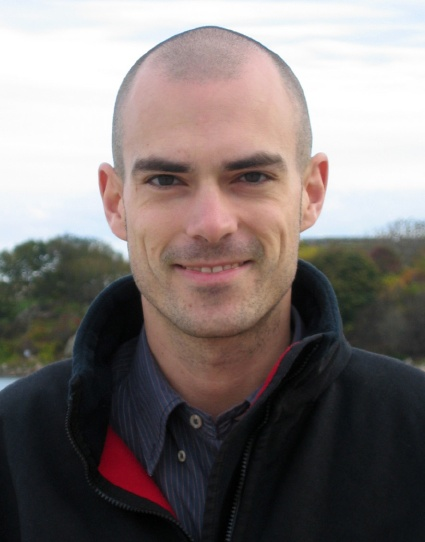
\includegraphics[width=1in,height=1.25in,clip,keepaspectratio]{pictures/oliverzahn.jpg}}]{Oliver Zahn}
Oliver Zahn is a computational/theoretical astrophysicist and the Executive Director of Berkeley Center for Cosmological Physics.
Trained as a multipurpose cosmologist, his research program tries to advance the understanding of the origin and evolution of structure in the Universe by applying a variety of analytical and numerical methods to complementary astrophysical observables.
\end{IEEEbiography}

\begin{IEEEbiography}[{\includegraphics[width=1in,height=1.25in,clip,keepaspectratio]{pictures/michaelfranklin.jpg}}]{Michael J. Franklin}
Michael J. Franklin is the Thomas M. Siebel Professor of Computer Science  the Director of the Algorithms, Machines, and People Laboratory (AMPLab) at UC Berkeley. Prof. Franklin is a co-PI and Executive Committee member for the Berkeley Institute of Data Science. He is a Fellow of the ACM and a two-time winner of the ACM SIGMOD "Test of Time" award.
\end{IEEEbiography}

\begin{IEEEbiography}[{\includegraphics[width=1in,height=1.25in,clip,keepaspectratio]{pictures/patterson.jpg}}]{David A. Patterson}
David Patterson is the E.H. and M.E. Pardee Professor of Computer Science at UC Berkeley and is a past president of ACM, and past chair of the UC Berkeley Computer Science Department. David has been awarded the IEEE von Neumann Medal, the IEEE Johnson Storage Award, the SIGMOD Test of Time award, the ACM-IEEE Eckert-Mauchly Award, and the Katayanagi Prize. He was also elected to both AAAS societies, the National Academy of Engineering, the National Academy of Sciences, the Silicon Valley Engineering Hall of Fame, and to be a Fellow of the Computer History Museum, the IEEE, and the ACM.
\end{IEEEbiography}

\begin{IEEEbiography}[{\includegraphics[width=1in,height=1.25in,clip,keepaspectratio]{pictures/saulperlmutter.jpg}}]{Saul Perlmutter}
Saul Perlmutter is an astrophysicist at the Lawrence Berkeley National Laboratory, a professor of physics at UC Berkeley, and the director of Berkeley Institute for Data Science. He is a member of the American Academy of Arts \& Sciences, a Fellow of the American Association for the Advancement of Science, and a member of the National Academy of Sciences. Along with Brian P. Schmidt and Adam Riess, Saul shared the 2006 Shaw Prize in Astronomy, the 2011 Nobel Prize in Physics, and the 2015 Breakthrough Prize in Fundamental Physics for the discovery of the accelerated expansion of the universe.
\end{IEEEbiography}

% insert where needed to balance the two columns on the last page with
% biographies
%\newpage

% You can push biographies down or up by placing
% a \vfill before or after them. The appropriate
% use of \vfill depends on what kind of text is
% on the last page and whether or not the columns
% are being equalized.

%\vfill

% Can be used to pull up biographies so that the bottom of the last one
% is flush with the other column.
%\enlargethispage{-5in}



% that's all folks
\end{document}


